% Options for packages loaded elsewhere
\PassOptionsToPackage{unicode}{hyperref}
\PassOptionsToPackage{hyphens}{url}
%
\documentclass[
]{article}
\usepackage{amsmath,amssymb}
\usepackage{lmodern}
\usepackage{ifxetex,ifluatex}
\ifnum 0\ifxetex 1\fi\ifluatex 1\fi=0 % if pdftex
  \usepackage[T1]{fontenc}
  \usepackage[utf8]{inputenc}
  \usepackage{textcomp} % provide euro and other symbols
\else % if luatex or xetex
  \usepackage{unicode-math}
  \defaultfontfeatures{Scale=MatchLowercase}
  \defaultfontfeatures[\rmfamily]{Ligatures=TeX,Scale=1}
\fi
% Use upquote if available, for straight quotes in verbatim environments
\IfFileExists{upquote.sty}{\usepackage{upquote}}{}
\IfFileExists{microtype.sty}{% use microtype if available
  \usepackage[]{microtype}
  \UseMicrotypeSet[protrusion]{basicmath} % disable protrusion for tt fonts
}{}
\makeatletter
\@ifundefined{KOMAClassName}{% if non-KOMA class
  \IfFileExists{parskip.sty}{%
    \usepackage{parskip}
  }{% else
    \setlength{\parindent}{0pt}
    \setlength{\parskip}{6pt plus 2pt minus 1pt}}
}{% if KOMA class
  \KOMAoptions{parskip=half}}
\makeatother
\usepackage{xcolor}
\IfFileExists{xurl.sty}{\usepackage{xurl}}{} % add URL line breaks if available
\IfFileExists{bookmark.sty}{\usepackage{bookmark}}{\usepackage{hyperref}}
\hypersetup{
  pdftitle={Exploring the composition of lithic assemblages in Mesolithic south-eastern Norway},
  pdfauthor={Isak Roalkvam1,},
  hidelinks,
  pdfcreator={LaTeX via pandoc}}
\urlstyle{same} % disable monospaced font for URLs
\usepackage[margin=1in]{geometry}
\usepackage{longtable,booktabs,array}
\usepackage{calc} % for calculating minipage widths
% Correct order of tables after \paragraph or \subparagraph
\usepackage{etoolbox}
\makeatletter
\patchcmd\longtable{\par}{\if@noskipsec\mbox{}\fi\par}{}{}
\makeatother
% Allow footnotes in longtable head/foot
\IfFileExists{footnotehyper.sty}{\usepackage{footnotehyper}}{\usepackage{footnote}}
\makesavenoteenv{longtable}
\usepackage{graphicx}
\makeatletter
\def\maxwidth{\ifdim\Gin@nat@width>\linewidth\linewidth\else\Gin@nat@width\fi}
\def\maxheight{\ifdim\Gin@nat@height>\textheight\textheight\else\Gin@nat@height\fi}
\makeatother
% Scale images if necessary, so that they will not overflow the page
% margins by default, and it is still possible to overwrite the defaults
% using explicit options in \includegraphics[width, height, ...]{}
\setkeys{Gin}{width=\maxwidth,height=\maxheight,keepaspectratio}
% Set default figure placement to htbp
\makeatletter
\def\fps@figure{htbp}
\makeatother
\setlength{\emergencystretch}{3em} % prevent overfull lines
\providecommand{\tightlist}{%
  \setlength{\itemsep}{0pt}\setlength{\parskip}{0pt}}
\setcounter{secnumdepth}{5}
\usepackage{amsmath}
\usepackage{booktabs}
\usepackage{caption}
\usepackage{longtable}
\ifluatex
  \usepackage{selnolig}  % disable illegal ligatures
\fi
\newlength{\cslhangindent}
\setlength{\cslhangindent}{1.5em}
\newlength{\csllabelwidth}
\setlength{\csllabelwidth}{3em}
\newenvironment{CSLReferences}[2] % #1 hanging-ident, #2 entry spacing
 {% don't indent paragraphs
  \setlength{\parindent}{0pt}
  % turn on hanging indent if param 1 is 1
  \ifodd #1 \everypar{\setlength{\hangindent}{\cslhangindent}}\ignorespaces\fi
  % set entry spacing
  \ifnum #2 > 0
  \setlength{\parskip}{#2\baselineskip}
  \fi
 }%
 {}
\usepackage{calc}
\newcommand{\CSLBlock}[1]{#1\hfill\break}
\newcommand{\CSLLeftMargin}[1]{\parbox[t]{\csllabelwidth}{#1}}
\newcommand{\CSLRightInline}[1]{\parbox[t]{\linewidth - \csllabelwidth}{#1}\break}
\newcommand{\CSLIndent}[1]{\hspace{\cslhangindent}#1}

\title{Exploring the composition of lithic assemblages in Mesolithic south-eastern Norway}
\author{Isak Roalkvam\textsuperscript{1,*}}
\date{09 May, 2021}

\begin{document}
\maketitle

{
\setcounter{tocdepth}{2}
\tableofcontents
}
\textsuperscript{1} University of Oslo

\textsuperscript{*} Correspondence: \href{mailto:isak.roalkvam@iakh.uio.no}{Isak Roalkvam \textless{}\href{mailto:isak.roalkvam@iakh.uio.no}{\nolinkurl{isak.roalkvam@iakh.uio.no}}\textgreater{}}

\begin{verbatim}
#> NULL
\end{verbatim}

\hypertarget{introduction}{%
\section{Introduction}\label{introduction}}

This study employs multivariate exploratory statistics to analyse the entirety of the lithic assemblages associated with a larger number of Mesolithic sites located in south-eastern Norway. This is done to identify latent patterns and structure in the relationship between the assemblages, with the ultimate aim of identifying behaviourally induced variation in their composition across time and space. However, the composition of the assemblages can be expected to be determined by a multitude of factors (e.g. Dibble et al., 2017), ranging from the impact of natural formation processes, to various and intermixed behavioural aspects such as purpose, duration, frequency and group sizes at visits to the sites. The assemblages are also likely to be impacted by variation in lithic technology, artefact function, use-life and discard patterns, as well as access to raw materials. Finally, analytical and methodological dimensions relating to survey, excavation and classification practices are also fundamental to how the assemblages are defined. Consequently, the analysis conducted here is done from an exploratory perspective, where all of these factors should be seen as potential contributors to any observed pattern.

However, even though each individual assemblage can have been impacted by an infinitude of effects that might skew an archaeological interpretation, this does not preclude the applicability of inductive analyses aimed at revealing overarching structure in the data, without imposing overly complex analytical frameworks that attempt to account for these particularities (Bevan, 2015). Structure that can be revealed from considering all of the assemblages in aggregate can constitute a step in an iterative analytical chain that ultimately aims to tease apart such aspects from the multitude of factors that have shaped the composition of the assemblages, and should be of value to subsequent in-depth studies of any individual site. The most immediate danger of the approach outlined here is rather to be overly naive in the causal significance and cultural importance that is ascribed to any identified pattern. As such, the main aim of this analysis is to compare the results with findings reported in previous literature concerned with the Mesolithic in southern Norway and have the generation of new hypotheses as a possible outcome. To this end, the analysis follows two analytical avenues. The first involves an analysis of the assemblages that is based on the classification of the artefacts done for the original excavation reports. The second involves an analysis of the assemblages in light of the whole assemblage behaviour index, which has not seen application in this context before.

\hypertarget{archaeological-context-and-material}{%
\subsection{Archaeological context and material}\label{archaeological-context-and-material}}

The 54 coastal sites chosen for analysis here have a relatively limited geographical distribution in south-eastern Norway \ref@(fig:dist)A{]}. The sites were excavated as part of four larger excavation projects that all took place within the last 15 years (\textbf{solheim2013b?}; \textbf{jaksland2014a?}; \textbf{melvold2014b?}; \textbf{reitan2014l?}; \textbf{solheim2017b?}). The sites included in the analysis consists of all Mesolithic sites excavated in conjunction with the projects that have assemblages holding more than 100 artefacts. The institution responsible for these excavations was the Museum of Cultural History in Oslo. This has led to a considerable overlap in the archaeological personnel involved, and comparable excavation practices across the excavations. Furthermore, with these projects, major efforts were made to standardise how lithic artefacts were to be classified at the museum. As a result, this should reduce the amount of artificial patterning in the data incurred by discrepancies in the employed systems for categorisation (e.g. Clark and Riel-Salvatore, 2006; Dibble et al., 2017). In this setting, for example, bias could potentially follow from the fact that two of the projects have sites with relatively contemporaneous dates (Jaksland, 2014, see also \ref@(fig:dist)B; \textbf{solheim2013b?}). Any project-dependent classification practice could as a consequence lead to an exaggeration of chronological differences between the assemblages. While this is difficult to fully account for, I do believe that the relative contemporaneity of the excavation projects, as well as the overlap in excavation and classification practices should minimise the above-mentioned effects, making the data-set a good candidate for exploratory data analysis.

\begin{figure}
\centering
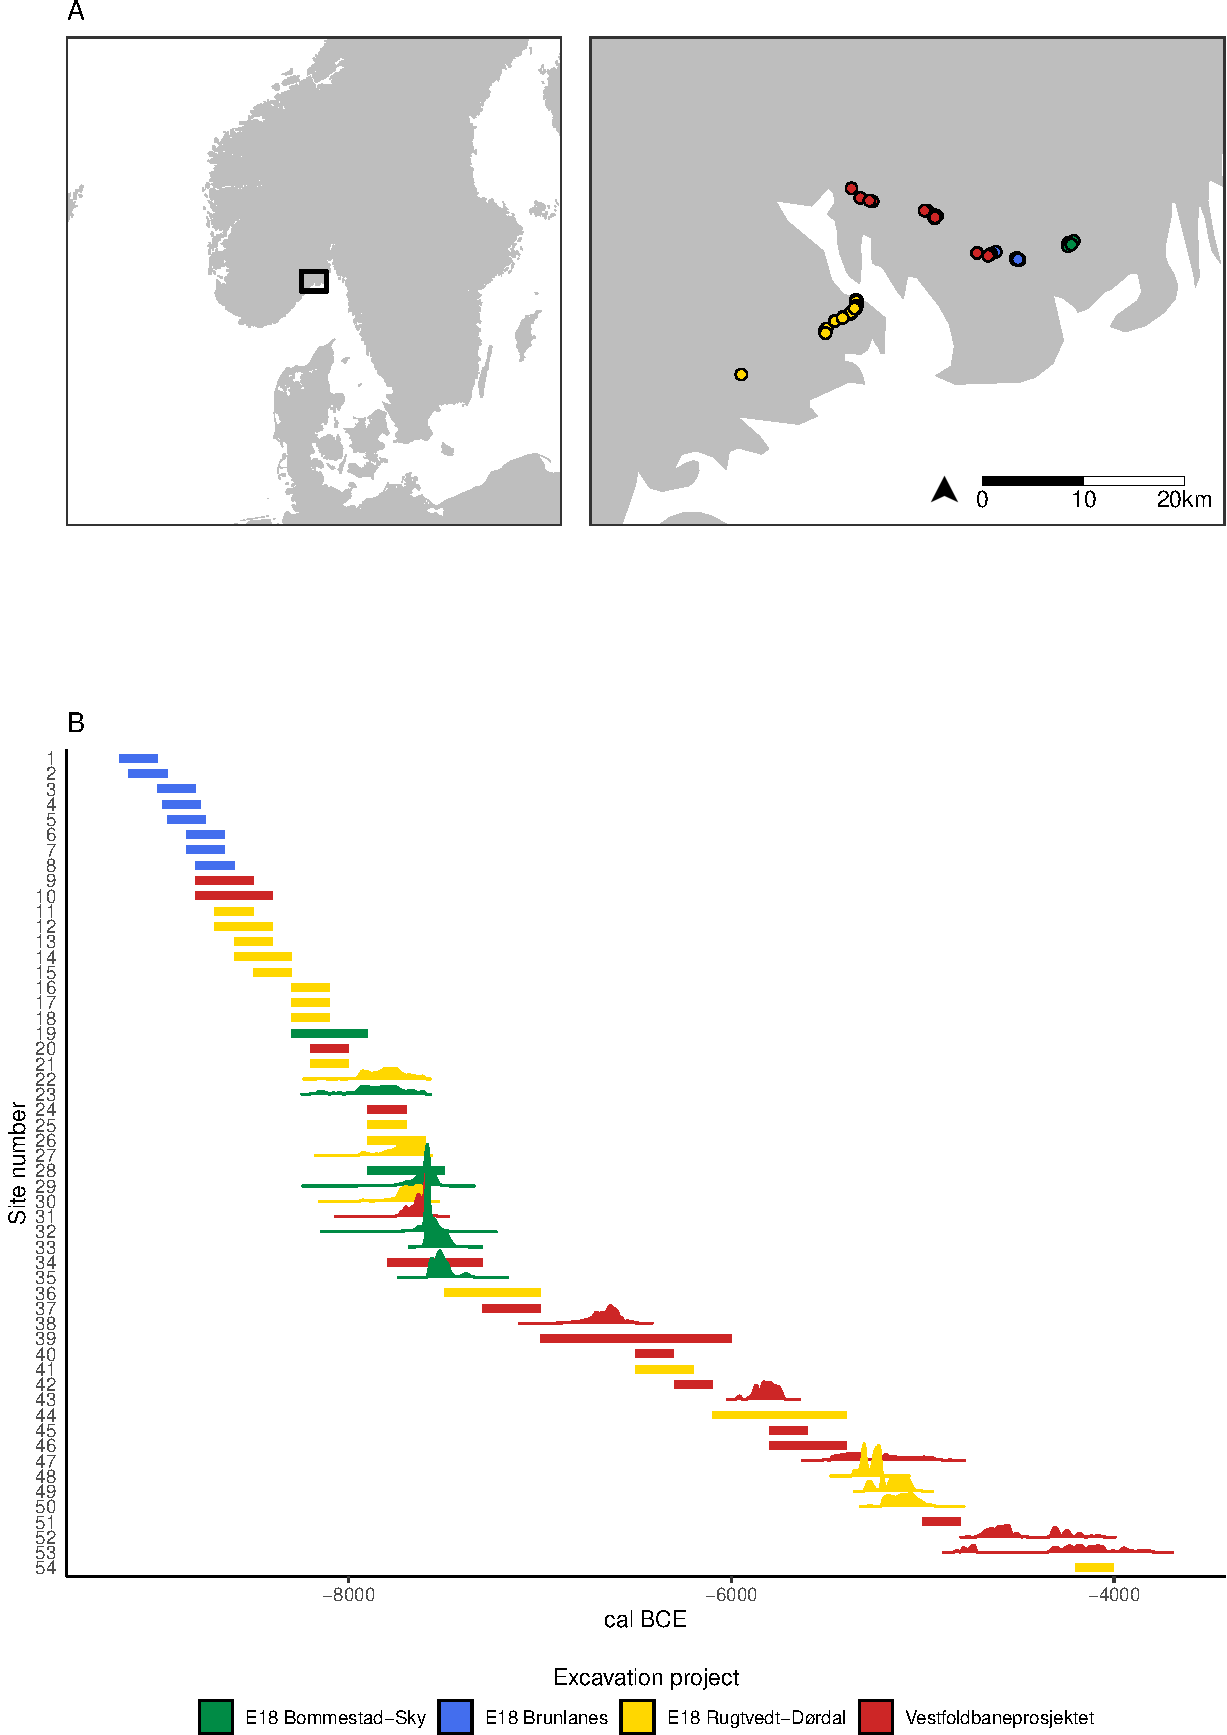
\includegraphics{../figures/dist-1.pdf}
\caption{\label{fig:dist}A) Spatial and B) temporal distribution of the sites chosen for analysis. Radiocarbon probability density functions are given as the posterior sum. Solid lines indicate that the site has been dated with reference to relative sea-level change and typological indicators. These follow the original reports.}
\end{figure}

A defining characteristic of the Norwegian Mesolithic is that a clear majority of the known sites are located in coastal areas (Glørstad, 2010). Furthermore, these coastal sites appear to predominantly have been located on or close to the contemporary shoreline when they were in use (Breivik et al., 2018; Solheim et al., 2020). In south-eastern Norway, this pattern is combined with a continuous regression of the shoreline, following from isostatic rebound (Romundset et al., 2018; e.g. Sørensen, 1979). The fairly rapid shoreline displacement means that the sites tend not to have retained their strategic or ecologically beneficial shore-bound location for long periods of time (cf. Perreault, 2019, p. 47). Consequently, the shore-bound settlement, combined with the rapid shoreline displacement has resulted in a relatively high degree of spatial separation of cumulative palimpsests, to follow the terminology of Bailey (2007), while shoreline displacement combined with shore-bound settlement allows for a relatively good chronological control of these accumulation events. In other parts of the world, a higher degree of spatial distribution means that while the physical separation of material can help delineate discrete events, this typically comes at the cost of loosing temporal resolution, as any stratigraphic relationship between the events is lost (Bailey, 2007). However, as the rate of isostatic rebound has varied throughout the Mesolithic in the region, and local topography and bathymetry will have impacted how rapidly a site lost its shore-bound location, this effect is not evenly distributed in time and space. In the earliest part of the Mesolithic, the displacement rate within the study area would have been around as much as 8.8 cm/year, falling to around 0.5 cm/year in the Late Mesolithic (Sørensen et al., 2014). Thus, while relative sea-level change appears to have reduced the degree of mixing that has occurred in the assemblages, this could vary depending on when and where they were in use, in turn potentially reducing the degree to which their composition can be directly compared --- a point that is returned to in the discussion of the results.

The data analysed here is based on the classification of the 54 site assemblages done for the original excavation reports, and consists of 48 variables representing different debitage and tool types. While the classification practices for the excavation projects were standardised to an extent, there are some instances where time was allocated to identify additional artefact sub-categories aimed at answering specific research questions. Some categories in the original reports have therefore been combined in the dataset. This for example pertains to the category narrow-blades, which is defined as blades of width between 8 and 12 mm. In the reports, this was only separated from (macro-)blades (width \(\ge\) 12 mm) and micro-blades (width \(\le\) 8 mm) for some of the sites. Narrow-blades were combined with the blade category here. Furthermore, the artefact data have here been divided into flint and non-flint materials. Flint does not occur indigenously in Norway, and is only available locally as nodules that have been transported and deposited by retreating and drifting ice (e.g. Berg-Hansen, 1999). This means that the distribution and quality of the flint has been impacted by a diverse set of factors relating to climatic and geographical factors such as, but not limited to, topographic variability, shoreline morphology and ocean currents (Eigeland, 2015, p. 46). An in depth-analysis of the flint quality from sevens sites did result in the finding that the flint quality was relatively high, and consistently so across the sites. However, despite flint being treated as a unified category here, the cited study by was based on only seven sites located some km distance from the present study area, meaning that the results might not necessarily be transferable to the sites treated here (Eigeland, 2015, pp. 45--53). Furthermore, the various non-flint raw materials that have been lumped together here can have quite disparate properties, where fine-grained cryptocrystalline materials are often used as a substitute or supplement to flint, while other, coarser materials are usually associated with the production of axes and other macro tools. Given this differentiated use, these raw-material properties are expected to be reflected in the retained debitage and tool categories. An important benefit of combining all of the non-flint materials is that this reduces the dependency on whether or not these have been correctly and consistently categorised for the reports (cf. Frivoll, 2017). While certainly a topic deserving of more attention, the general sentiment in the literature is that there would have been stable access to locally available non-flint raw-materials of good quality in south-eastern Norway (Eigeland, 2015, p. 370).

Previous studies of lithic artefacts in Norway have typically had a focus on chronological trends associated with formal tool types (e.g. Helskog et al., 1976; Reitan, 2016), involved refit-studies of the entirety of individual assemblages (Skar and Coulson, 1986), or been concerned with technological processes associated with certain sub-categories of the site inventories, such as blades or axes (e.g. Damlien, 2016; Solheim et al., 2020). Some studies have involved in-depth analyses of handful of sites in terms of intrasite spatial organisation (Nærøy, 2018), and technological organisation {[}Eigeland (2015); Mansrud and Eymundsson (2016);{]}. There are also some more comprehensive evaluations of a larger number of entire lithic assemblages to get at potential site types and associated mobility patterns (Breivik, 2020; \textbf{breivik2016?}; \textbf{viken2018c?}). However, the narratively driven analyses of these data makes the weighting of different variables unclear, and these studies draw their conclusions based on an arguably over-constraining predefined trichotomy of site types. Each site could have had complex life histories and been associated with a wide range of tasks that in sum make up the assemblages. Finally, only a single study concerned with eight Middle-Mesolithic assemblages --- assemblages that are also treated here --- has employed a multivariate quantitative framework to help structure such a treatment (\textbf{solheim2013?}). In sum, therefore, previous studies are typically either limited to a small number of sites, to a subset of the inventories, or to more subjectively and narratively driven methods.

In a series of case studies from Northern Norway, Bølviken et al. (1982) were among a group of scholars often attributed the popularisaton of correspondence analysis (CA) in wider archaeologcal circles (Baxter, 1994). In southern Norway, however, the use of multivariate statistics in Mesolithic research is to my knowledge limited to (\textbf{solheim2013a?}) use of CA to analyse the assemblage data from eight sites excavated in connection with a development-led project. As these sites, which are included in this study, have relatively contemporaneous dates, the Solheims analysis was mainly aimed at identifying potential variation in the

There have been a few studies that have conducted comprehensive analyses of artefact inventories and site features to get at variation in Mesolithic site types (Breivik, 2020; Viken, 2018). As Binford originally clarified, a point that has also been retiterated by several authors since; these categories are best understood as extremes on a continuous scale.

\hypertarget{methods}{%
\subsection{Methods}\label{methods}}

The first part of the analysis conducted here involves employing the method of correspondence analysis (CA), using the lithic count data as classified for the original excavation reports. The purpose of this exercise is to evaluate the degree to which the composition of the assemblages align with patterns that have been suggested by earlier studies that have employed more informally driven methods when the entirety of the assemblages are taken into account. This consequently assumes that the artefact categories employed in Norwegian Stone Age archaeology are, at least to a certain extent, behaviorally meaningful. However, the approach taken is also partially informed by the so-called Frison effect (Jelinek, 1976), which pertains to the fact that lithics studied by archaeologists can have had long and complex use-lives in which they took on a multitude of different shapes before they were ultimately discarded. Several scholars have built on this to argue that morphological variation in retouched lithics cannot be assumed to predominantly be the result of the intention of the original knapper to reach some desired end-product, but rather that what is commonly categorised as discrete types of artefacts by archaeologists can instead in large part be related to variable degrees of modification through use and rejuvination (e.g. Barton, 1991; Dibble, 1995). Consequently, several artefact categories have here been collapased for the CA. This for example pertains to tool types such as scrapers, burins, drills, knives and otherwise indeterminate artefacts with retouch. That these categories are internally consistent and categorically exclusive in terms of fulfilled purpose is at best a dubious proposition, in turn potentially rendering their contribution as discrete analytic units misleading. These have all been combined into the single category ``small flint tools.'' (A full overview of the aggregated variables and their constituent parts is provided in the supplementary material). While aggregating artefact categories in this manner could potentially subsume important variation, it does also reduce the possibility that any conclusions are not simply the result of employing erroneous units of analysis. An underlying assumption is therefore that the retained categories represent artefact categories that have fulfilled different purposes or are related to different technological processes. While ultimately intuitive in nature, it does seem reasonable to assume that for example large non-flint stone tools such as axes, adzes, chisels, clubs and hatches, here categorised as non-flint macro tools, have fulfilled different purposes than the previously mentioned small flint tools.

However, the fact that for the most part we lack even a most basic understanding of what any individual lithic object has been used for does have major implications that the above-outlined analysis does not take properly into account, and renders it difficult to align any identified patterns with specific behavioural dimensions (Dibble et al., 2017). For example, a vast amount of artefacts defined as debitage are likely to have fulfilled the function of tools, and both debitage and formal tool types could have had various different purposes and had a multitude of shapes throughout their use-life. While use-wear analysis could potentially offer a way to identify what artefacts were used for towards the end of their use-life, these kinds of analyses are extremely time-consuming and are therefore typically only conducted on a smaller number of artefacts that have already been selected for analysis based on their shape (e.g. Solheim et al., 2018). Thus, while these analyses can potentially get at in-group variation pertaining to the end-state of a group of artefacts, they do not tell us whether or not their classification as a unified group is meaningful in the first place (Dibble et al., 2017). As a consequence, the second part of the analysis employs a suite of measures developed for the classification of lithic assemblages developed with these inferential limitations in mind (see Clark and Barton, 2017, and below). The logic behind these measures are founded on an understanding of technology as being organised along a continuum ranging between curated and expedient (Binford, 1979). An expedient technological organisation pertains to the situational production of tools to meet immediate needs, with little investment of time and resources in modification and rejuvination, resulting in high rates of tool replacement. Curated technological organisation, on the other hand, has been defined as related to manufacture and maintenance of tools in anticipation of future use, the transport of these artefacts between places of use, and the modification and rejuvenation of artefacts for different and changing situations (Binford, 1979). Although precisely how it is measured may vary, the empirical correspondent to a curated technological organisation is therefore typically defined by high degrees of retouch, as this is commonly seen as a means of realising the potential utility of a tool or extending its use-life by the repeated rejuvination and modification of edges (e.g. Bamforth, 1986; Dibble, 1995; Shott and Sillitoe, 2005). The continuum between curated and expedient technology has in turn been related to land-use and mobility strategies, as well as raw-material quality and availability (Andrefsky, 1994; Clark and Barton, 2017; Kuhn, 1992; e.g. Parry and Kelly, 1987; Smith, 2015).

While the definition of curation, its archaeological correlates, and behavioural implications have been widely discussed Shott (1996), following not least from the ambiguous definition first put forward by Binford (1979), some concrete operationalisation of the terms have been suggested. Through a series of studies Barton and collegues (e.g. 1999; Barton and Riel-Salvatore, 2014; Clark and Barton, 2017) have shown that the relationship between lithic volumetric density and relative frequency of retouched artefacts provide consistent results across a wide range of chronological and cultural context. This measure is taken to reflect degree of curation associated with the assemblages, which in turn is mainly to follow from variation in mobility patterns associated with the sites (Barton and Riel-Salvatore, 2014). Higher degree of mobility would mean a higher dependency on the artefacts and the material people could bring with them, and dimensions such as weight, reliabilty, repairability, and the degree to which artefacts could be manipulated to fulfill a wide range of tasks are therefore assumed to have been factors of concern. From this it follows that the empirical expectation for short-term camps is a curated technological organisation with higher relative frequency of retouched artefacts, and a lower overall density of lithics (Clark and Barton, 2017). More time spent in a single location, on the other hand, is in this model assumed to lead to better control of raw-material availability and to allow for its accumulation. This should in turn lead to an expedient technological organisation with reduced necessity for the conservation of lithics and extensive use of retouch. The empirical expectation for lower degree of mobility is therefore relatively high density of lithics and a low relative frequency of retouched artefacts. A further empirical expectation of an expendient tehcnological organisation is as a consequence also a higher number of cores and unretouched flakes and blades (Clark and Barton, 2017).

This is the main measure employed here. Some additional variables suggested by Bicho and Cascalheira (2020) to be related to mobility patterns are subsequently also explored using principal components analysis (PCA), following the continuous operationalisations of these measures (cf. Baxter, 1994, p. 100).

A note should also be made on the fact that a couple of variables that are sometimes invoked for the classification of sites in terms of associated mobility pattern are omitted here. This pertains to number of site features such as fireplaces, cooking pits and dwelling structures. Feature count has been omitted as taphonomic loss is likely to lead to a chronological bias in their preservation. Similarly, the number of activity areas, effectively number artefact clusters, however defined, has also been disregarded. This follows most notably from the fact that the impact of post-depositional processes at Stone Age sites in Norway is arguably understudied. This pertains for example to the impact of bioturbation in the form of three-throws, which can can have a detrimental effect on the original distribution of artefacts, and which can be expected to have been relatively frequent on several of the sites treated here (Jørgensen, 2017; \textbf{darmark2018e?}).

Within this framework, amount of retouch has been seen as a empirical indicator of degree of curation. While various methods for measuring the curation associated with individual tools have been forwarded, the approach taken here focuses on the assemblage considered as a whole.

Here retouch i At logistical basecamps, the extended time spent in a single location would imply a better control of raw material availability, and allow for longer trips to retrieve these. Higher availability of lithic raw materials should in turn reduce the necessity for extensive retouch, meaning the material expectation for logistical basecamps would be relatively high density of lithics and a low relative frequency of retouched artefacts. From this it follows that the empirical expectation for short-term camps is a higher relative frequency of retouched artefacts, and a lower overall density of lithics (Clark and Barton, 2017).

\hypertarget{theorycalculation}{%
\section{Theory/calculation}\label{theorycalculation}}

Higher frequency of secondarily worked lithics

\hypertarget{results}{%
\section{Results}\label{results}}

\begin{figure}
\centering
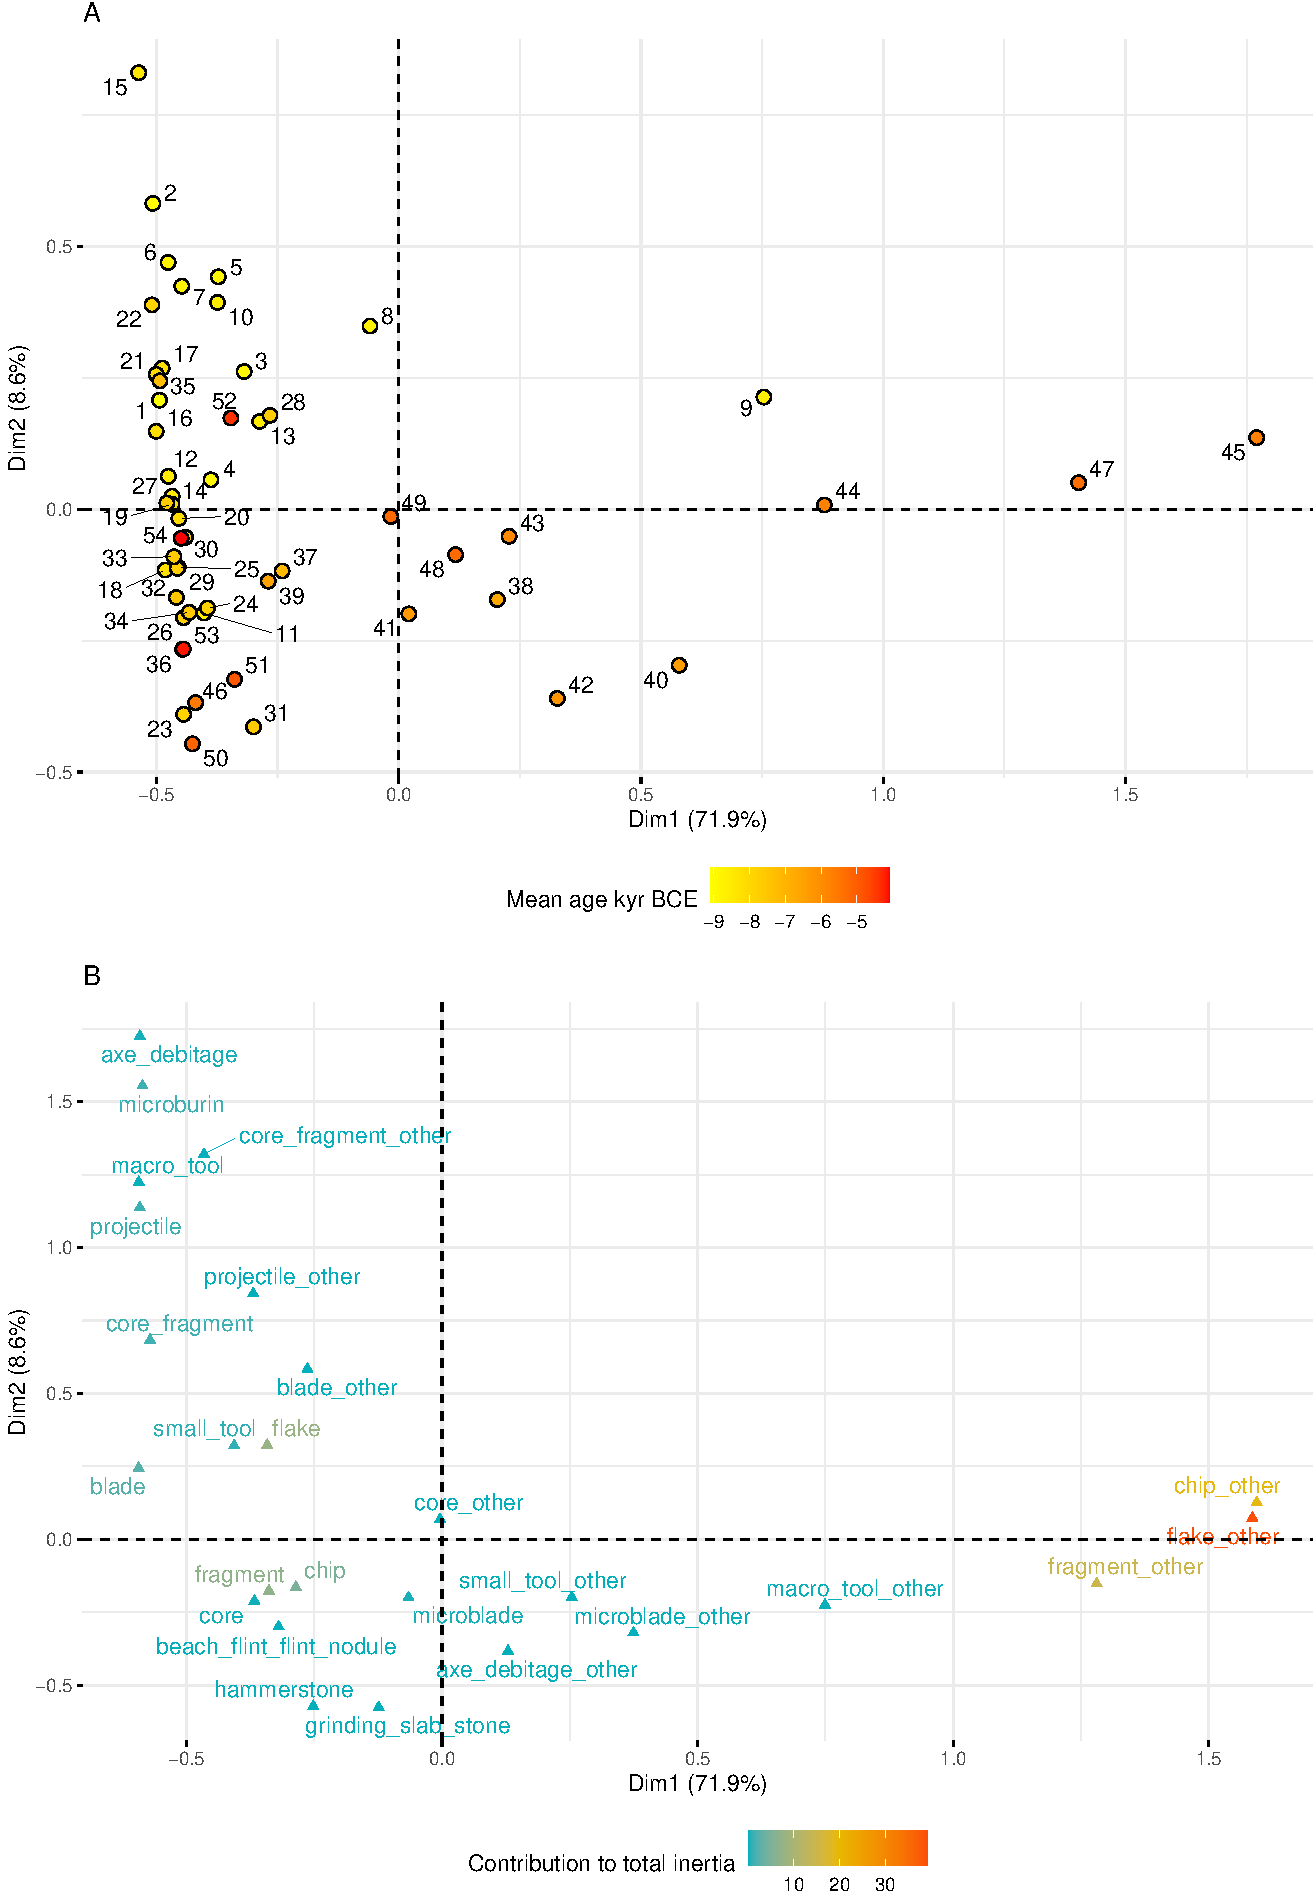
\includegraphics{../figures/cor-1.pdf}
\caption{\label{fig:cor}Correspondence analysis using artefact count data. A) Object map, B) Variable map.}
\end{figure}

Figure \ref{fig:cor} displays the CA using the lithic count data. While no clear-cut clusters can be readily delineated, the general impression from the plots is that a chronological dimension is associated with the patterning in the data. This is indicated by the general transition across the colour scale in the row plot (Figure \ref{fig:cor}A), combined with the fact that the two first dimensions of the CA accounts for as much as 80.53 \% of the inertia or variance in the data. The earliest sites tend to be located in the upper right corner of plot A, with increasingly younger sites towards the bottom along the second dimension. Although fewer in number, the sites from the later parts of the Mesolithic are drawn out along the first dimension of the plot, and are not as impacted by the second dimension as the more numerous older sites.

The column plot (Figure \ref{fig:cor}B) reveals that the earliest sites are characterised by the flint artefact categories microburins, projectiles, as well as flint macro tools and associated debitage. It is also interesting that these sites to larger extent are characerised by core fragments, both in flint and non-flint materials, than cores themselves. The non-flint material on the earliest sites appears to be centered around the production of projectiles, as both the projectiles themselves and non-flint blades are important constituents of the assemblages at these sites. These findings are in large part in line with previous research (e.g. Bang-Andersen, 2003), although possibly highlighting the importance of the non-flint materials to a larger extent than what has traditionally been the case.

The first dimension, which is pulling some of the later sites towards the right of the plot, is mainly defined by macro tools and associated debitage in non-flint materials that are negatively correlated with more flint dominated assemblages and non-flint projectiles. While the outer end of the first dimensions is dominated by later Mesolithic sites associated with axe production in non-flint materials, the later sites occur along the entire dimension, indicating that while these axe production sites are a feature of the later Mesolithic, there is marked variation among these later sites. Although the sample size is quite strained and the discussion of finer chronological points might not be warranted, the first dimension does appear to be of of less importance for the absolute latest sites, as indicated by their location to the left of the plot. This could indicate that specialised axe production sites disappear towards the end of the Mesolithic, a notion that would be in line with previous research Glørstad (2011).

In addition, Nedre Hobekk 2 represents a somewhat curious case in that its assemblage is dominated by axe production in metarhyolite. The use of metarhyolite is typically seen as a feature of the end of the EM and the MM, but is evidently not as prominent a part of other sites that are contemporaneous with Nedre Hobekk 2.

\hypertarget{section}{%
\section{}\label{section}}

Reducing the number of such inferential leaps by aggregating artefact groups could potentially subsume important variation, but it does also reduce the possibility that the conclusions of any analysis is not simply the result of the employed units of analysis, and an overly naive trust in the fact that these units reflect any behaviourally meaningful categories. This realisation has led to a wide range of outside Scandinavian Mesolithic research, meaning a range of empirical measures associated with various mobility patterns are available.

It has, however, been suggested that access to raw-materials can be a more important decider for assemblage composition than mobility patterns , and that variable workability of these materials will impact factors such as the relative frequency of tools to debitage in the assemblages (e.g. Andrefsky, 1994; Manninen and Knutsson, 2014). In addition to attempts at accounting for this analytically (see below), the limited geographical distribution of the sites should alleviate the issue somewhat, as the overall availability of raw materials could be expected to be more comparable through time than if a wider region was under consideration.

Of these the most well-estbalished is the. base don the assumption that, this measure and has been shown to display a meaningful measure across a wide range of temporal, geographical and cultural contexts.

\begin{figure}
\centering
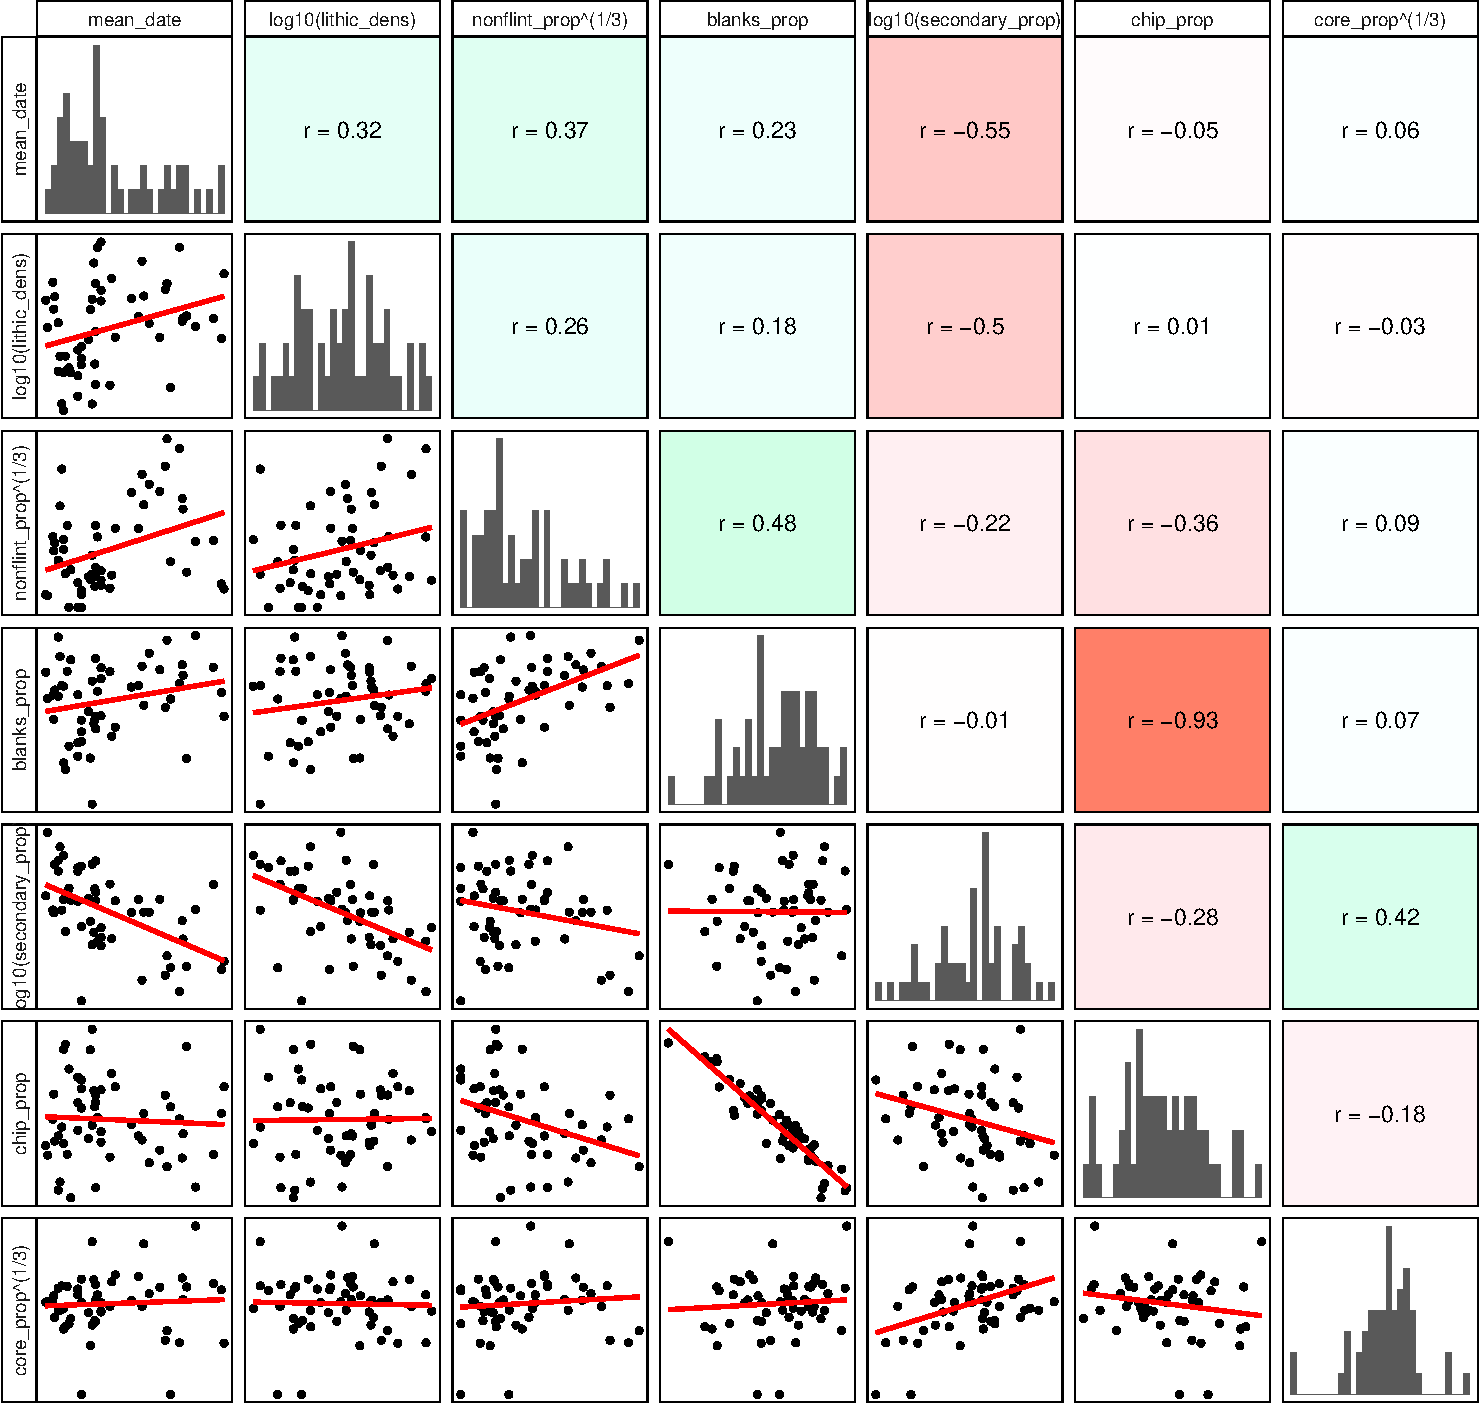
\includegraphics{../figures/cor-plot-1.pdf}
\caption{\label{fig:cor-plot}Correlation plot showing transformation of skewed variables for the PCA, and the linear correlation between these}
\end{figure}

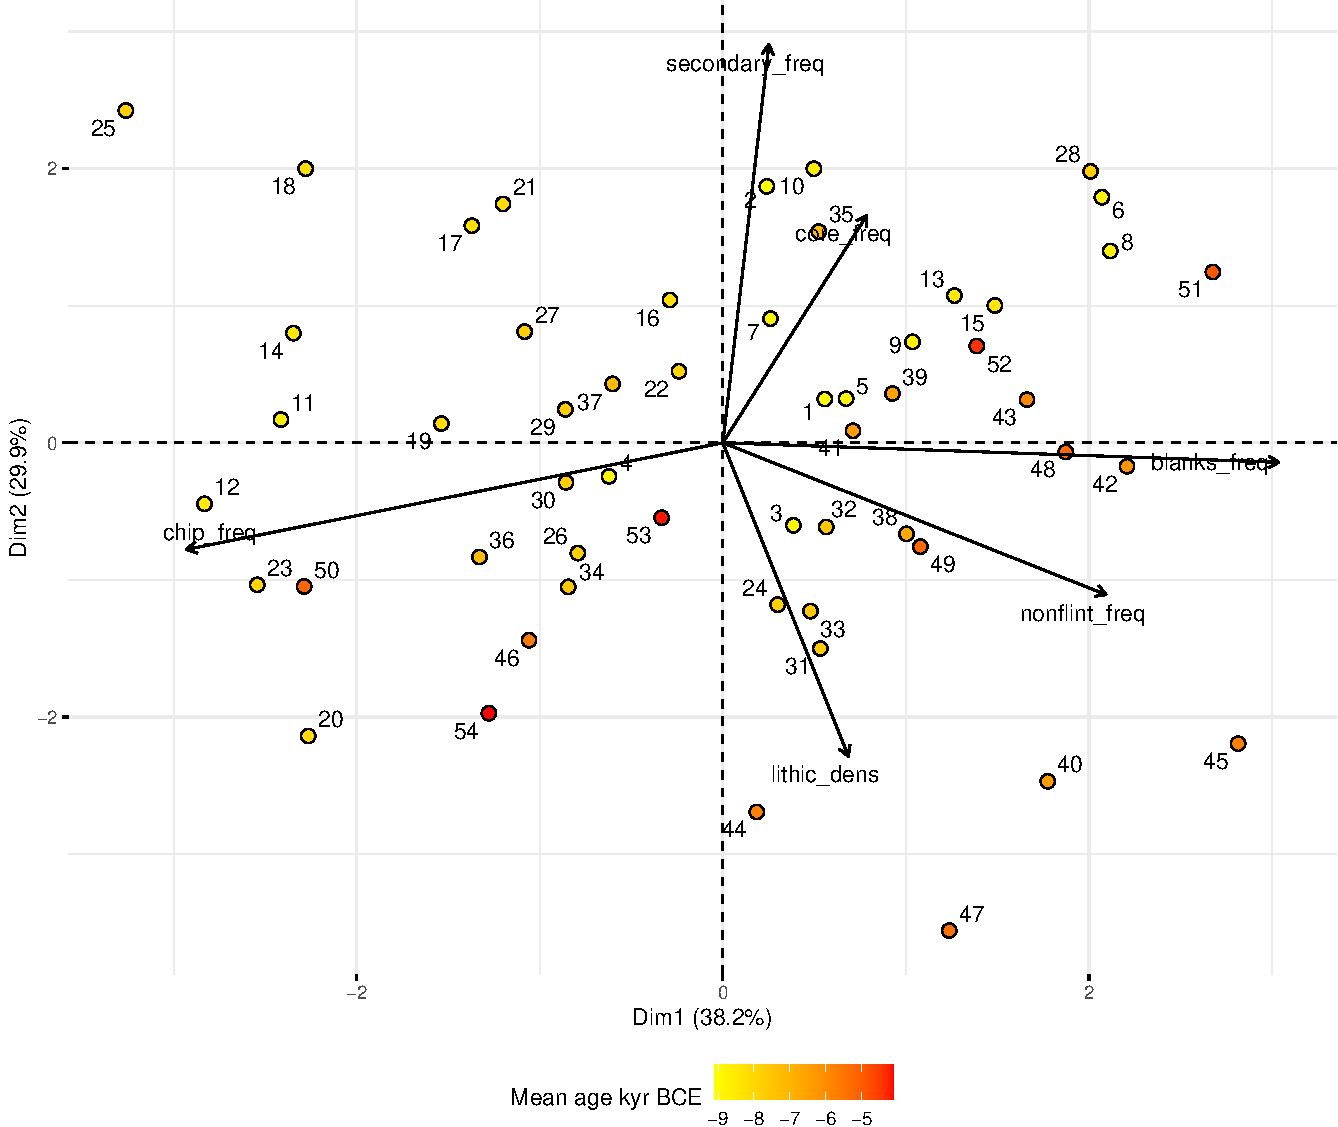
\includegraphics{../figures/pca-analysis-1.pdf}
Figure \ref{fig:pca-analysis} displays a principle components analysis using variations of the continuous measures for mobility patterns as operationalised by Clark and Barton (2017) and Bicho and Cascalheira (2020). While the investigation performed by Bicho and Cascalheira (2020) indicates that the relative frequency of chips, cores, and blanks might be more sensitive to mobility patterns, they also found that the relationship between volumetric density of lithics and the frequency of retouched artefacts gave a reasonable estimation of mobility in their data. hese last dimensions are capturing the most variation in the dataset presented here. Thus, if frequency of secondarily worked artefacts and volumetric density of lithics is accepted as a proxy for degree of mobility, these findings would consequently be in line with previous research into the Mesolithic of Norway, indicating that earlier sites are associated with higher degree of mobility than sites from later phases. Furthermore, the fact that these

\captionsetup[table]{labelformat=empty,skip=1pt}
\begin{longtable}{cccc}
\toprule
Component & Eigenvalue & Variance (\%) & Cumulative variance (\%) \\ 
\midrule
1 & 2.29 & 38.21 & 38.21 \\ 
2 & 1.79 & 29.90 & 68.11 \\ 
3 & 0.95 & 15.85 & 83.96 \\ 
4 & 0.62 & 10.32 & 94.28 \\ 
5 & 0.32 & 5.39 & 99.66 \\ 
6 & 0.02 & 0.34 & 100.00 \\ 
\bottomrule
\end{longtable}

\begin{figure}
\centering
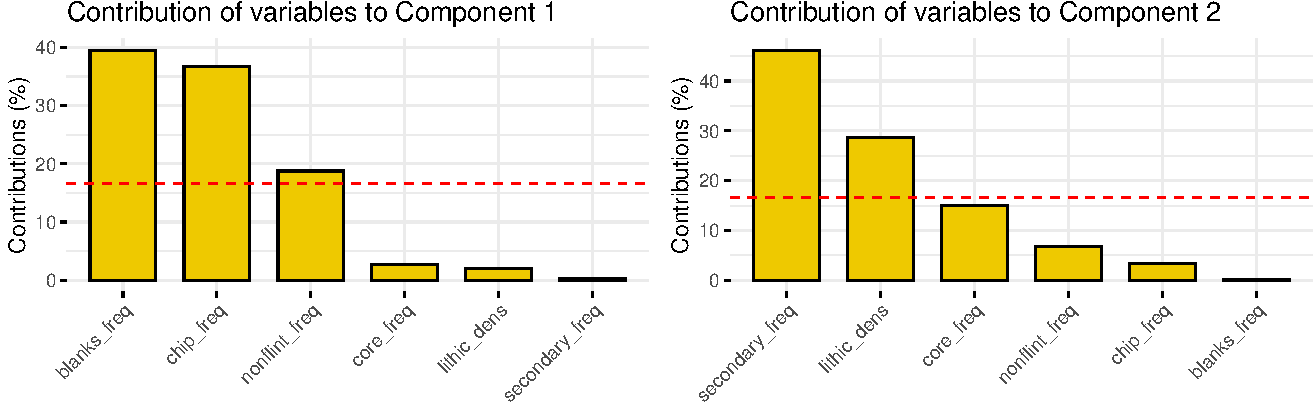
\includegraphics{../figures/var_contrib-1.pdf}
\caption{(\#fig:var\_contrib)Contribution of variables to components.}
\end{figure}

Figure \ref{fig:wabi} displays the WABI as found for the site data. This indicates a negative correlation between the two variables (r = -0.5) and a general tendency for younger sites to be associated with a higher volumetric density of lithics and a lower relative frequency of secondarily worked lithics than older sites. Following Clark and Barton (2017), this would be in line with a general transition from a expedient to curated lithic technology. Variable raw-material availability can also impact these measures as (Manninen and Knutsson, 2014). Variation in raw-material use over time could consequently mean that these patterns could be an effect of the available raw material rather than mobility strategies. However, as is evident in when considering both plots in \ref{fig:wabi}, the pattern is evident for both the lithics considered in aggregate and for the flint data specifically. Although the distribution is slightly more spread out along the y-axis than the x-axis in the flint data, indicating that differences in volumtric density of flint is not as clearly chronologically, the general pattern is the same.

To visualise this temporal trend more clearly, a curation index based on the two variables was devised by performing a min-max normalisation of the two variables, scaling them to take on values between 0 and 1. The values for artefact density was then made negative to reflect its relationship with degree of curation. The mean was then found for each site on these two normalised values. To account for the temporal uncertainty associated with the sites, a simulation based approach was also adopted. A LOESS curve was fit to the data for each simulation, where the age of each site was drawn from the date ranges associated with the sites. For sites with radiocarbon age determinations the dates were drawn from the associated posterior probability density functions, while ages for sites dated with reference to relative sea-level change and typology were drawn uniformly from the associated date ranges. This simulation was repeated 5000 times, the results of which is visualed in . Disregarding the edge-effects at either end of the plot, the general tendency is a relatively high degree of curation among the earlier sites, which then has a marked drop around 8000 BCE before remaining relatively stable until the end of the Mesolithic. It is also interseting that the variation in degree of curation is higher after 8000 BCE, potentially reflecting variation in site types and associated mobility patterns. Plotting the results indicates a higher degree of curation among the earliest sites, which then falls and settles without any further major fluctuations.

\begin{figure}
\centering
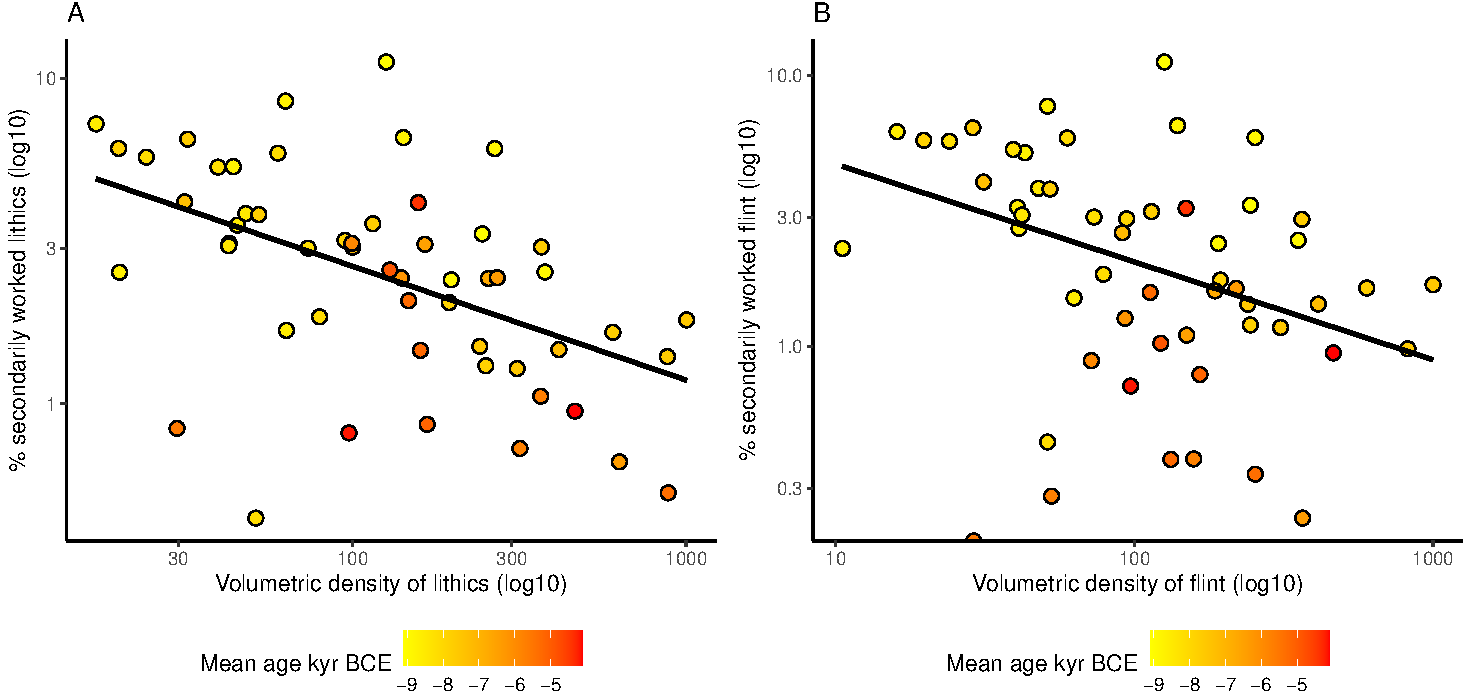
\includegraphics{../figures/wabi-1.pdf}
\caption{\label{fig:wabi}Relative frequency of secondarily worked lithics plotted against the volumetric density of artefacts (artefact count / excavated m\textsuperscript{3}) for A) All lithics, B) Flint. The logarithm is taken to base 10 on all axes.}
\end{figure}

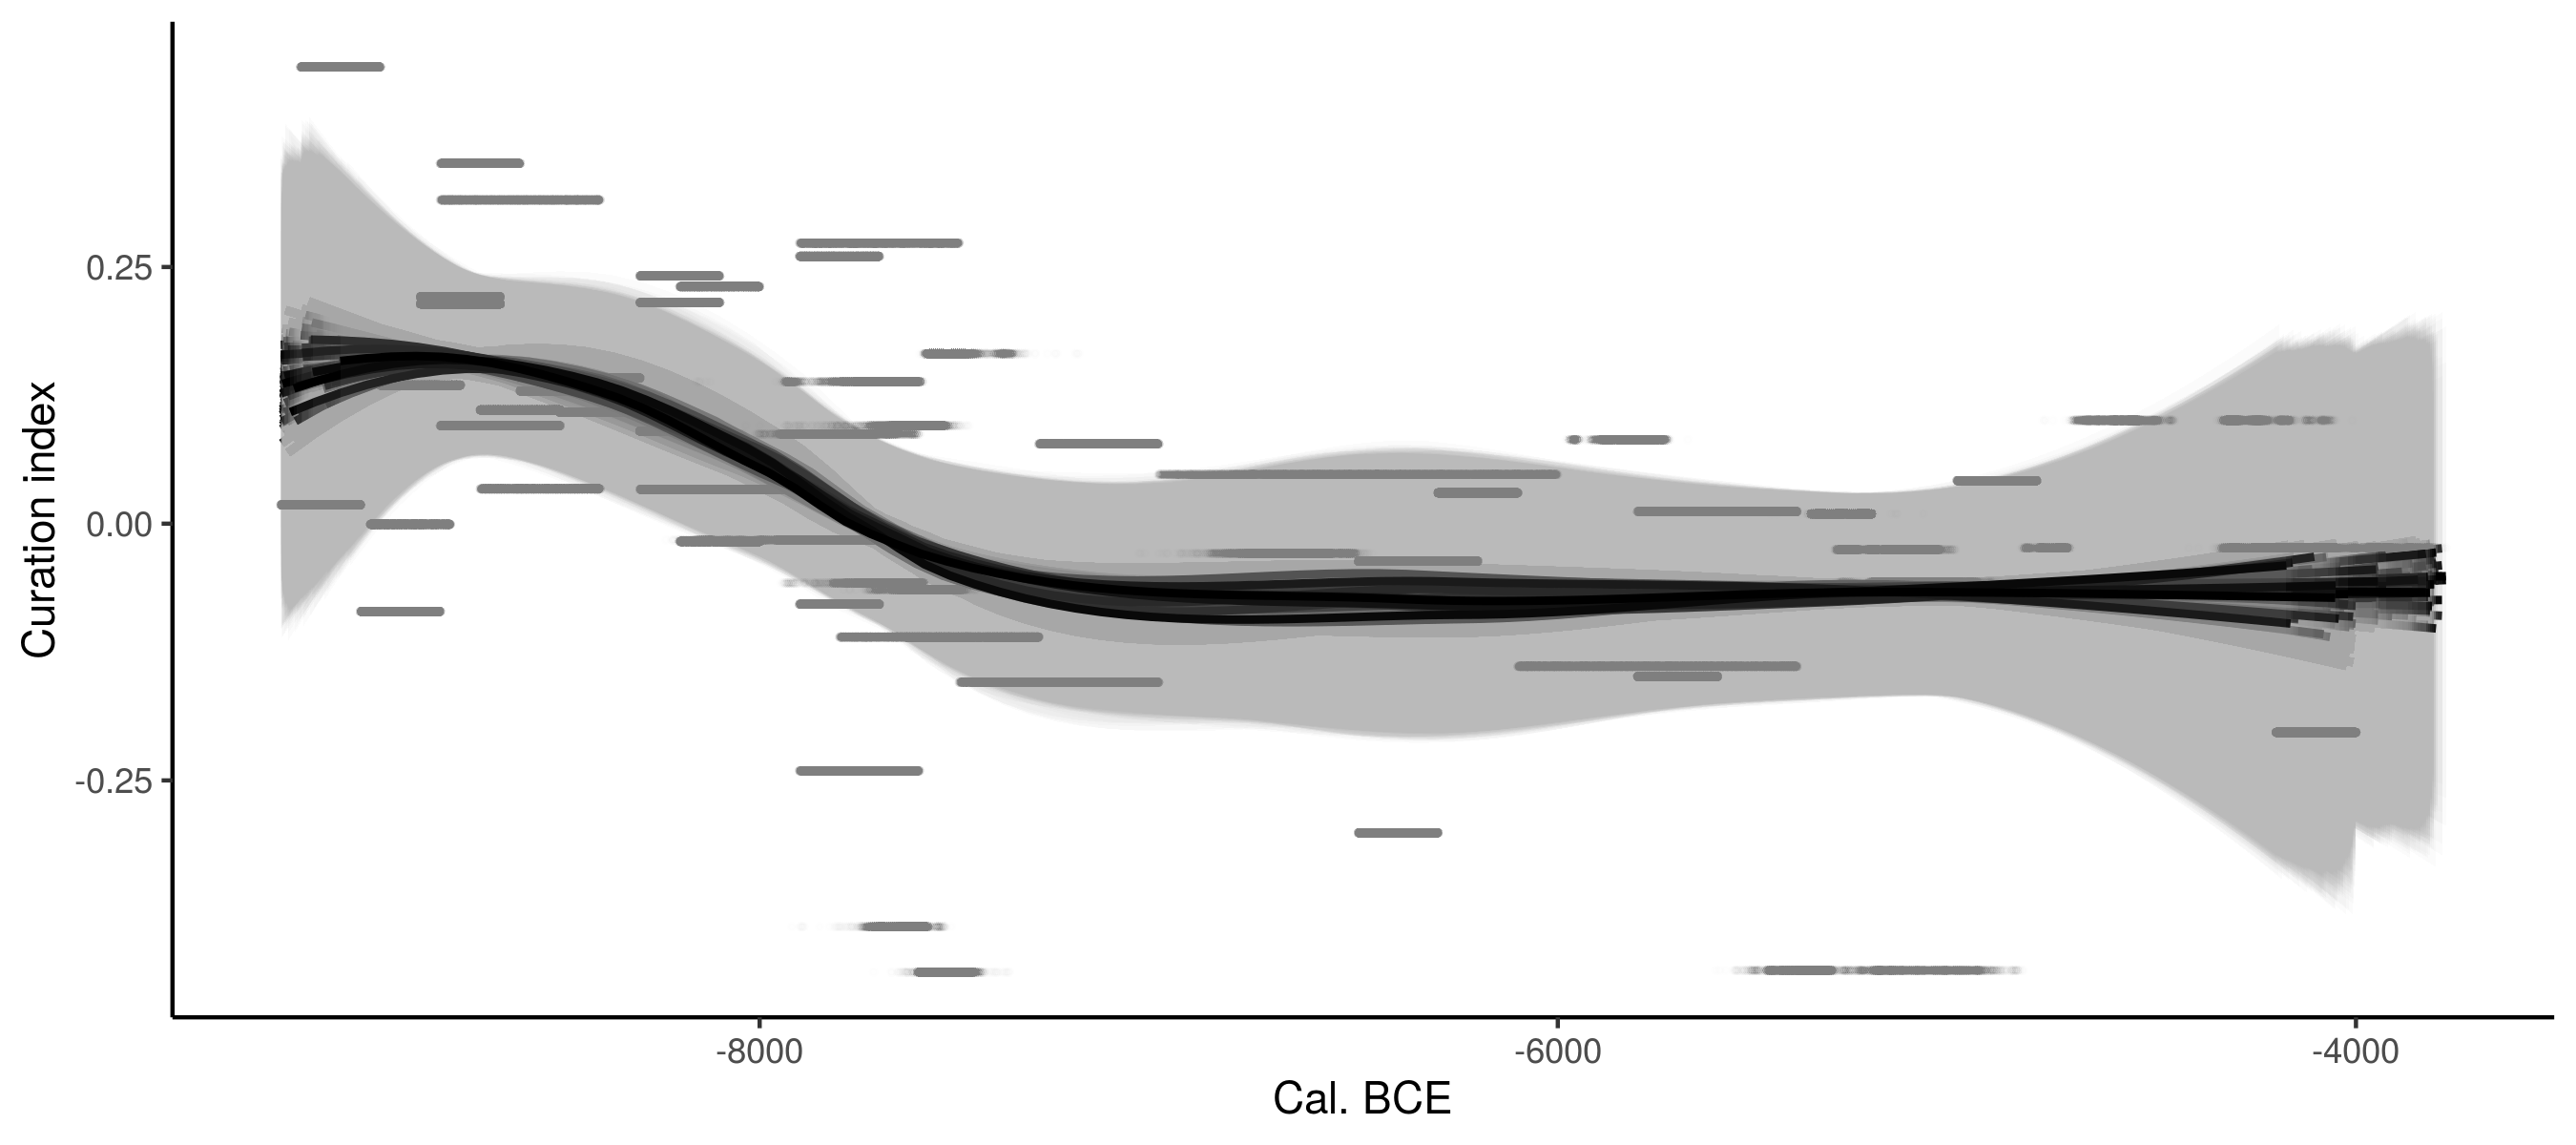
\includegraphics{../figures/simage-1.pdf}

\hypertarget{discussion}{%
\section{Discussion}\label{discussion}}

The results of the CA does appear to align reasonably well with previous research that has been based on more informal analyses of artefact types, indicating that the employed artefact categories are capturing some behaviorally meaningful patterning that changes over time. However, as several authors have pointed out in relation to the application of CA for seriation purposes, `time is not the only dimension.' The developments evident here do also most certainly correspond to more pervasive cultural change than a purely typo-chronological development of artefact morphology, highlighted perhaps most clearly by the influence of the later Mesolithic axe production sites. Unpicking and aligning the signficance of these chronological patterns with any specific behavioural dimensions using the CA results is, however, another task entirely. This follows most clearly from the fact that for the most part we lack even a most basic understanding of what any individual lithic object has been used for, leaving the behavioural significance of the employed units of analysis unclear (see section, above).

these results do speak to the cross-cultural and cross-temporal applicability of the measure, and consequently the potential it holds for comparative studies. The findings indicated by the WABI, as well as by the negative correlation between relative frequency of primarily and secondarily worked lithics, do align more clearly with previous suggestions concerning the overall mobility patterns in Mesolithic Norway. However, the question then becomes: What is the significance of the negatively correlated variables of relative frequency of cores and chips? Given that these are more or less orthogonal to the WABI variables on the first and second component, this would indicate that if one of these variable pairs is taken to reflect the scale between expedient and curated technologies, it should follow that the other variable pair is not correlated with these. As the entire temporal range of the sites is spread out between the extremes of the chip and core variables, one possibility is that these are indicative of site types that are temporally ubiquitous. In attempt to determine if this might be the case, it was decided to introduce site locational data from a previous study that in addition to surveyed sites involved the analysis of the sites treated here Roalkvam (2020). Of the variables considered, this study found that the most consistently important environmental covariates for the location of sites in the region was related to the exposure of the sites, and failed to identify any diachronic variation in this pattern. As it has previously been proposed that sites located in areas exposed to wind and waves and with large overview of surrounding areas is a characteristic of hunting stations or similarly temporary , one could envisage that variablity in site functionality might be reflected in degree of exposure. However, introducing these variables does not clarify the picture, as both variables show negligible degrees of correlation with any of the variables pertaining to the assemblage data.

This is arguably more established than the variables included bysimilarities between the variable plots of Bicho and Cascalheira (2020) and the variables indicated in is striking. This pertains to the negative correlation between core and chip frequency, and the negative correlation between primary and secondarily worked lithics. This last

These measures are taken from the framework of whole assemblage behavioural index, as developed by , and is aimed to get at behavioural dimensions relating to mobility patterns among hunter-gatherers.

\hypertarget{conclusion}{%
\section{Conclusion}\label{conclusion}}

The results of the CA using the entirety of the lithic assemblages align more or less with results of previous research in south-eastern Norway. This would indicate that in general, meaningful chronological patterning is associated with the employed artefact categories. These tendencies are already well-established when it comes to formal tool types, but the have been given less focus in terms of entire assemblages these notions have previously Precisely what behavioural implication the development in the use of these types have, however, is unclear

The results of considering variables that are have been associated with mobility patterns gave rise to two competing hypotheses. These pertain to whether the degree of curation associated with the assemblages as captured by the changing ratio of primary to secondarily worked lithics over time is the result of changing raw material availability or mobility patterns. The orthogonal relationship between core to chip frequency would in this framework be expected to be capturing the opposite relationship. If degree of curation mainly reflects changes in raw-material quality and availability, this would then indicate that mobility patterns are comparable throughout the Mesolithic as the core to chip frequency is not time-dependent. And vice verca --- if the changing mobility patterns is the main driver of the transition from curated to expedient technological organisation, as operationalised here, While this would be in line with findings from a recent evaluation of the locational patterns associated with the sites (Roalkvam, 2020), there is no readily available empirical evidence, no smoking gun, se findings are the results of an exploratory analysis, and are therefore perhaps best seen as potentially laying the framework for later targeted strategic test of these competing hypotheses.

\newpage

\hypertarget{references}{%
\section{References}\label{references}}

\hypertarget{refs}{}
\begin{CSLReferences}{1}{0}
\leavevmode\hypertarget{ref-andrefsky1994}{}%
Andrefsky, W., 1994. Raw-material availability and the organization of technology. American Antiquity 59, 21--34. \url{https://doi.org/10.2307/3085499}

\leavevmode\hypertarget{ref-bailey2007}{}%
Bailey, G., 2007. Time perspectives, palimpsests and the archaeology of time. Journal of Anthropological Archaeology 26, 198--223. \url{https://doi.org/10.1016/j.jaa.2006.08.002}

\leavevmode\hypertarget{ref-bamforth1986}{}%
Bamforth, D.B., 1986. Technological Efficiency and Tool Curation. American Antiquity 51, 38--50. \url{https://doi.org/10.2307/280392}

\leavevmode\hypertarget{ref-bang-andersen2003}{}%
Bang-Andersen, S., 2003. Southwest Norway at the Pleistocene/Holocene Transition: Landscape Development, Colonization, Site Types, Settlement Patterns. Norwegian Archaeological Review 36, 5--25. \url{https://doi.org/10.1080/00293650307293}

\leavevmode\hypertarget{ref-barton1991}{}%
Barton, C.M., 1991. Retouched Tools, Fact or Fiction? Paradigms for Interpreting Paleolithic Chipped Stone, in: Clark, G.A. (Ed.),. University of Pennsylvania Press, pp. 143--163.

\leavevmode\hypertarget{ref-barton1999}{}%
Barton, C.M., Bernabeu, J., Aura, J.E., García, O., 1999. Land-Use Dynamics and Socioeconomic Change: An Example from the Polop Alto Valley. American Antiquity 64, 609--634. \url{https://doi.org/10.2307/2694208}

\leavevmode\hypertarget{ref-barton2014}{}%
Barton, C.M., Riel-Salvatore, J., 2014. The formation of lithic assemblages. Journal of Archaeological Science 46, 334--352. \url{https://doi.org/10.1016/j.jas.2014.03.031}

\leavevmode\hypertarget{ref-baxter1994}{}%
Baxter, M.J., 1994. Exploratory multivariate analysis in archaeology. Percheron Press, New York.

\leavevmode\hypertarget{ref-berg-hansen1999}{}%
Berg-Hansen, I.M., 1999. The availability of flint at lista and jæren, southwestern norway, in: Boaz, J. (Ed.),. University of Oslo, Oslo, pp. 255--266.

\leavevmode\hypertarget{ref-bevan2015}{}%
Bevan, A., 2015. The data deluge. Antiquity 89, 1473--1484. \url{https://doi.org/10.15184/aqy.2015.102}

\leavevmode\hypertarget{ref-Bicho2020}{}%
Bicho, N., Cascalheira, J., 2020. Use of lithic assemblages for the definition of short-term occupations in hunter-gatherer prehistory, in: Cascalheira, J., Picin, A. (Eds.),. Springer, Cham, p. 1938. \url{https://doi.org/10.1007/978-3-030-27403-0₂}

\leavevmode\hypertarget{ref-binford1979}{}%
Binford, L.R., 1979. Organization and Formation Processes: Looking at Curated Technologies. Journal of Anthropological Research 35, 255--273.

\leavevmode\hypertarget{ref-breivik2020}{}%
Breivik, H.M., 2020. Diachronic trends among early mesolithic sites types? A study from the coast of central norway, in: Schülke, A. (Ed.),. Rutledge, London \& New York, pp. 121--146.

\leavevmode\hypertarget{ref-breivik2018}{}%
Breivik, H.M., Fossum, G., Solheim, S., 2018. Exploring human responses to climatic fluctuations and environmental diversity: Two stories from Mesolithic Norway. Quaternary International, Impacts of gradual and abrupt environmental changes on Late glacial to Middle Holocene cultural changes in Europe 465, 258--275. \url{https://doi.org/10.1016/j.quaint.2016.12.019}

\leavevmode\hypertarget{ref-buxf8lviken1982}{}%
Bølviken, E., Helskog, E., Helskog, K., Holm-Olsen, I.M., Solheim, L., Bertelsen, R., 1982. Correspondence analysis: An alternative to principal components. World Archaeology 14, 41--60. \url{https://doi.org/10.1080/00438243.1982.9979848}

\leavevmode\hypertarget{ref-clark2017}{}%
Clark, G.A., Barton, C.M., 2017. Lithics, landscapes \& la Longue-durée {{}} Curation \& expediency as expressions of forager mobility. Quaternary International, Prehistoric hunter-gatherers and farmers in the Adriatic and neighboring regions 450, 137--149. \url{https://doi.org/10.1016/j.quaint.2016.08.002}

\leavevmode\hypertarget{ref-clark2006}{}%
Clark, G.A., Riel-Salvatore, J., 2006. Observations on systematics in paleolithic archaeology, in: Hovers, E., Kuhn, S. (Eds.),. Springer, New York, pp. 29--56.

\leavevmode\hypertarget{ref-damlien2016}{}%
Damlien, H., 2016. Eastern pioneers in westernmost territories? Current perspectives on Mesolithic hunter{{}}gatherer large-scale interaction and migration within Northern Eurasia. Quaternary International, Holocene Hunter-Gatherer Archaeology of Northern Eurasia (Guest Editors: Peter Jordan and Andrzej Weber) 419, 5--16. \url{https://doi.org/10.1016/j.quaint.2014.02.023}

\leavevmode\hypertarget{ref-dibble1995}{}%
Dibble, H.L., 1995. Middle paleolithic scraper reduction: Background, clarification, and review of the evidence to date. Journal of Archaeological Method and Theory 2, 299--368. \url{https://doi.org/10.1007/BF02229003}

\leavevmode\hypertarget{ref-dibble2017}{}%
Dibble, H.L., Holdaway, S.J., Lin, S.C., Braun, D.R., Douglass, M.J., Iovita, R., McPherron, S.P., Olszewski, D.I., Sandgathe, D., 2017. Major Fallacies Surrounding Stone Artifacts and Assemblages. Journal of Archaeological Method and Theory 24, 813--851. \url{https://doi.org/10.1007/s10816-016-9297-8}

\leavevmode\hypertarget{ref-eigeland2015}{}%
Eigeland, L., 2015. Maskinmennesket i steinalderen. Endring og kontinuitet i steinteknologi fram mot neolitiseringen av øst-norge (PhD thesis). Oslo.

\leavevmode\hypertarget{ref-frivoll2017}{}%
Frivoll, A., 2017. Identifisering og klassifisering av littiske råmaterialer i sør- og østnorsk steinalderforskning. Reliabilitet av visuell klassifiseringsmetode (PhD thesis). Oslo.

\leavevmode\hypertarget{ref-gluxf8rstad2011}{}%
Glørstad, H., 2011. The Nøstvet axe, in: Davis, V., Edmonds, M. (Eds.),. Oxbow Books, pp. 21--36.

\leavevmode\hypertarget{ref-gluxf8rstad2010}{}%
Glørstad, H., 2010. The structure and history of the late mesolithic societies in the oslo fjord area 6300-3800 BC. Bricoleur Press, Lindome.

\leavevmode\hypertarget{ref-helskog1976}{}%
Helskog, K., Indrelid, S., Mikkelsen, E., 1976. Morfologisk klassifisering av slåtte steinartefakter. Universitetets Oldsaksamling Årbok 1972-74, 9--40.

\leavevmode\hypertarget{ref-jaksland2014}{}%
Jaksland, L., 2014. Kulturhistorisk sammenstilling, in: Jaksland, L., Persson, P. (Eds.),. Museum of Cultural History, University of Oslo, Oslo, pp. 11--46.

\leavevmode\hypertarget{ref-jelinek1976}{}%
Jelinek, A.J., 1976. Form, function and style in lithic analysis, in: Cleland, C.E. (Ed.),. Academic Press, New York, pp. 19--33.

\leavevmode\hypertarget{ref-juxf8rgensen2017}{}%
Jørgensen, E.K., 2017. Om vegetasjonsforstyrrelser: Konsekvenser for bevaringen av arkeologisk kontekstinformasjon i norske jordsmonn. Viking 80, 157180--157180. \url{https://doi.org/10.5617/viking.5477}

\leavevmode\hypertarget{ref-kuhn1992}{}%
Kuhn, S.L., 1992. On Planning and Curated Technologies in the Middle Paleolithic. Journal of Anthropological Research 48, 185--214.

\leavevmode\hypertarget{ref-manninen2014}{}%
Manninen, M.A., Knutsson, K., 2014. Lithic raw material diversification as an adaptive strategy{{}}Technology, mobility, and site structure in Late Mesolithic northernmost Europe. Journal of Anthropological Archaeology 33, 84--98. \url{https://doi.org/10.1016/j.jaa.2013.12.001}

\leavevmode\hypertarget{ref-mansrud2016}{}%
Mansrud, A., Eymundsson, C., 2016. Socialized landscapes? Lithic clusters, hearths and relocation rituals at Middle Mesolithic sites in Eastern Norway. Fennoscandia archaeologica 33, 27--55.

\leavevmode\hypertarget{ref-nuxe6ruxf8y2018}{}%
Nærøy, A.J., 2018. Early Mesolithic spatial conformity in southern Norway. Journal of Archaeological Science: Reports 18, 905--912. \url{https://doi.org/10.1016/j.jasrep.2017.10.021}

\leavevmode\hypertarget{ref-parry1987}{}%
Parry, W.J., Kelly, R.L., 1987. Expedient core technology and sedentism, in: Johnson, J.K., Morrow, C.A. (Eds.),. Westview Press, Boulder \& London, pp. 285--308.

\leavevmode\hypertarget{ref-perreault2019}{}%
Perreault, C., 2019. The quality of the archaeological record. The University of Chicago Press, Chicago \& London.

\leavevmode\hypertarget{ref-reitan2016}{}%
Reitan, G., 2016. Mesolittisk kronologi i Sørøst-Norge {{}} et forslag til justering. Viking 79, 23--51. \url{https://doi.org/10.5617/viking.3903}

\leavevmode\hypertarget{ref-roalkvam2020}{}%
Roalkvam, I., 2020. Algorithmic Classification and Statistical Modelling of Coastal Settlement Patterns in Mesolithic South-Eastern Norway. Journal of Computer Applications in Archaeology 3, 288307. \url{https://doi.org/10.5334/jcaa.60}

\leavevmode\hypertarget{ref-romundset2018}{}%
Romundset, A., Lakeman, T.R., Høgaas, F., 2018. Quantifying variable rates of postglacial relative sea level fall from a cluster of 24 isolation basins in southern Norway. Quaternary Science Reviews 197, 175--192. \url{https://doi.org/10.1016/j.quascirev.2018.07.041}

\leavevmode\hypertarget{ref-shott1996}{}%
Shott, M.J., 1996. An Exegesis of the Curation Concept. Journal of Anthropological Research 52, 259--280. \url{https://doi.org/10.1086/jar.52.3.3630085}

\leavevmode\hypertarget{ref-shott2005}{}%
Shott, M.J., Sillitoe, P., 2005. Use life and curation in New Guinea experimental used flakes. Journal of Archaeological Science 32, 653--663. \url{https://doi.org/10.1016/j.jas.2004.11.012}

\leavevmode\hypertarget{ref-skar1986}{}%
Skar, B., Coulson, S., 1986. Evidence of behaviour from refitting - a case study. Norwegian Archaeological Review 19, 90--102.

\leavevmode\hypertarget{ref-smith2015}{}%
Smith, G.M., 2015. Modeling the influences of raw material availability and functional efficiency on obsidian projectile point curation: A Great Basin example. Journal of Archaeological Science: Reports 3, 112--121. \url{https://doi.org/10.1016/j.jasrep.2015.06.010}

\leavevmode\hypertarget{ref-solheim2020}{}%
Solheim, S., Damlien, H., Fossum, G., 2020. Technological transitions and human-environment interactions in Mesolithic southeastern Norway, 11~500{{}}6000~cal. BP. Quaternary Science Reviews 246, 106501. \url{https://doi.org/10.1016/j.quascirev.2020.106501}

\leavevmode\hypertarget{ref-solheim2018}{}%
Solheim, S., Fossum, G., Knutsson, H., 2018. Use-wear analysis of Early Mesolithic flake axes from South-eastern Norway. Journal of Archaeological Science: Reports 17, 560--570. \url{https://doi.org/10.1016/j.jasrep.2017.12.017}

\leavevmode\hypertarget{ref-suxf8rensen1979}{}%
Sørensen, R., 1979. Late Weichselian deglaciation in the Oslofjord area, south Norway. Boreas 8, 241--246. https://doi.org/\url{https://doi.org/10.1111/j.1502-3885.1979.tb00806.x}

\leavevmode\hypertarget{ref-suxf8rensen2014}{}%
Sørensen, R., Henningsmoen, K.E., Høeg, H.I., Gälman, V., 2014. Holocene landhevningsstudier i søndre vestfold og sørøstre telemark- revidert kurve, in: Melvold, S., Persson, P. (Eds.),. Portal, Kristiansand, pp. 36--47.

\leavevmode\hypertarget{ref-viken2018}{}%
Viken, S., 2018. Sagene B1. En tidligmesolittisk basisboplass med én boligstruktur og spor etter flere samtidige hushold, in: Reitan, G., Sundström, L. (Eds.),. Cappelen Damm Akademisk, Oslo, pp. 131--166.

\end{CSLReferences}

\newpage

\hypertarget{colophon}{%
\subsubsection{Colophon}\label{colophon}}

This report was generated on 2021-05-09 12:32:08 using the following computational environment and dependencies:

\begin{verbatim}
#> - Session info ---------------------------------------------------------------
#>  setting  value                       
#>  version  R version 4.0.5 (2021-03-31)
#>  os       Linux Mint 19.3             
#>  system   x86_64, linux-gnu           
#>  ui       X11                         
#>  language en_US                       
#>  collate  en_US.UTF-8                 
#>  ctype    en_US.UTF-8                 
#>  tz       Europe/Oslo                 
#>  date     2021-05-09                  
#> 
#> - Packages -------------------------------------------------------------------
#>  package       * version  date       lib source        
#>  abind           1.4-5    2016-07-21 [1] CRAN (R 4.0.3)
#>  assertthat      0.2.1    2019-03-21 [1] CRAN (R 4.0.3)
#>  backports       1.2.0    2020-11-02 [1] CRAN (R 4.0.3)
#>  bitops          1.0-6    2013-08-17 [1] CRAN (R 4.0.3)
#>  bookdown        0.21     2020-10-13 [1] CRAN (R 4.0.3)
#>  broom           0.7.3    2020-12-16 [1] CRAN (R 4.0.3)
#>  callr           3.5.1    2020-10-13 [1] CRAN (R 4.0.3)
#>  car             3.0-10   2020-09-29 [1] CRAN (R 4.0.3)
#>  carData         3.0-4    2020-05-22 [1] CRAN (R 4.0.3)
#>  cellranger      1.1.0    2016-07-27 [1] CRAN (R 4.0.3)
#>  checkmate       2.0.0    2020-02-06 [1] CRAN (R 4.0.3)
#>  class           7.3-18   2021-01-24 [4] CRAN (R 4.0.3)
#>  classInt        0.4-3    2020-04-07 [1] CRAN (R 4.0.3)
#>  cli             2.2.0    2020-11-20 [1] CRAN (R 4.0.3)
#>  cluster         2.1.2    2021-04-17 [4] CRAN (R 4.0.5)
#>  codetools       0.2-18   2020-11-04 [4] CRAN (R 4.0.3)
#>  colorspace      1.4-1    2019-03-18 [1] CRAN (R 4.0.3)
#>  crayon          1.3.4    2017-09-16 [1] CRAN (R 4.0.3)
#>  curl            4.3      2019-12-02 [1] CRAN (R 4.0.3)
#>  data.table      1.14.0   2021-02-21 [1] CRAN (R 4.0.5)
#>  DBI             1.1.0    2019-12-15 [1] CRAN (R 4.0.3)
#>  dbplyr          2.0.0    2020-11-03 [1] CRAN (R 4.0.3)
#>  desc            1.2.0    2018-05-01 [1] CRAN (R 4.0.3)
#>  devtools        2.3.2    2020-09-18 [1] CRAN (R 4.0.3)
#>  digest          0.6.27   2020-10-24 [1] CRAN (R 4.0.3)
#>  dplyr         * 1.0.2    2020-08-18 [1] CRAN (R 4.0.3)
#>  DT              0.16     2020-10-13 [1] CRAN (R 4.0.3)
#>  e1071           1.7-4    2020-10-14 [1] CRAN (R 4.0.3)
#>  ellipsis        0.3.1    2020-05-15 [1] CRAN (R 4.0.3)
#>  evaluate        0.14     2019-05-28 [1] CRAN (R 4.0.3)
#>  factoextra    * 1.0.7    2020-04-01 [1] CRAN (R 4.0.3)
#>  FactoMineR    * 2.4      2020-12-11 [1] CRAN (R 4.0.3)
#>  fansi           0.4.1    2020-01-08 [1] CRAN (R 4.0.3)
#>  farver          2.0.3    2020-01-16 [1] CRAN (R 4.0.3)
#>  flashClust      1.01-2   2012-08-21 [1] CRAN (R 4.0.3)
#>  forcats       * 0.5.0    2020-03-01 [1] CRAN (R 4.0.3)
#>  foreign         0.8-81   2020-12-22 [4] CRAN (R 4.0.3)
#>  fs              1.5.0    2020-07-31 [1] CRAN (R 4.0.3)
#>  generics        0.1.0    2020-10-31 [1] CRAN (R 4.0.3)
#>  GGally        * 2.1.1    2021-03-08 [1] CRAN (R 4.0.5)
#>  ggmap           3.0.0    2019-02-05 [1] CRAN (R 4.0.4)
#>  ggplot2       * 3.3.2    2020-06-19 [1] CRAN (R 4.0.3)
#>  ggpubr          0.4.0    2020-06-27 [1] CRAN (R 4.0.3)
#>  ggrepel         0.9.1    2021-01-15 [1] CRAN (R 4.0.3)
#>  ggridges      * 0.5.2    2020-01-12 [1] CRAN (R 4.0.3)
#>  ggsignif        0.6.0    2019-08-08 [1] CRAN (R 4.0.3)
#>  ggsn            0.5.0    2019-02-18 [1] CRAN (R 4.0.4)
#>  glue            1.4.2    2020-08-27 [1] CRAN (R 4.0.3)
#>  gt            * 0.2.2    2020-08-05 [1] CRAN (R 4.0.3)
#>  gtable          0.3.0    2019-03-25 [1] CRAN (R 4.0.3)
#>  haven           2.3.1    2020-06-01 [1] CRAN (R 4.0.3)
#>  here            1.0.0    2020-11-15 [1] CRAN (R 4.0.3)
#>  highr           0.8      2019-03-20 [1] CRAN (R 4.0.3)
#>  hms             0.5.3    2020-01-08 [1] CRAN (R 4.0.3)
#>  htmltools       0.5.0    2020-06-16 [1] CRAN (R 4.0.3)
#>  htmlwidgets     1.5.2    2020-10-03 [1] CRAN (R 4.0.3)
#>  httr            1.4.2    2020-07-20 [1] CRAN (R 4.0.3)
#>  jpeg            0.1-8.1  2019-10-24 [1] CRAN (R 4.0.3)
#>  jsonlite        1.7.1    2020-09-07 [1] CRAN (R 4.0.3)
#>  KernSmooth      2.23-18  2020-10-29 [1] CRAN (R 4.0.3)
#>  knitr           1.30     2020-09-22 [1] CRAN (R 4.0.3)
#>  labeling        0.4.2    2020-10-20 [1] CRAN (R 4.0.3)
#>  lattice         0.20-41  2020-04-02 [1] CRAN (R 4.0.3)
#>  leaps           3.1      2020-01-16 [1] CRAN (R 4.0.3)
#>  lifecycle       0.2.0    2020-03-06 [1] CRAN (R 4.0.3)
#>  lubridate       1.7.9.2  2020-11-13 [1] CRAN (R 4.0.3)
#>  magrittr        2.0.1    2020-11-17 [1] CRAN (R 4.0.3)
#>  maptools        1.0-2    2020-08-24 [1] CRAN (R 4.0.3)
#>  MASS            7.3-53.1 2021-02-12 [4] CRAN (R 4.0.3)
#>  Matrix          1.3-2    2021-01-06 [4] CRAN (R 4.0.3)
#>  memoise         1.1.0    2017-04-21 [1] CRAN (R 4.0.3)
#>  mgcv            1.8-33   2020-08-27 [1] CRAN (R 4.0.3)
#>  modelr          0.1.8    2020-05-19 [1] CRAN (R 4.0.3)
#>  munsell         0.5.0    2018-06-12 [1] CRAN (R 4.0.3)
#>  nlme            3.1-152  2021-02-04 [4] CRAN (R 4.0.3)
#>  openxlsx        4.2.3    2020-10-27 [1] CRAN (R 4.0.3)
#>  oxcAAR        * 1.1.0    2021-02-23 [1] CRAN (R 4.0.5)
#>  patchwork     * 1.1.0    2020-11-09 [1] CRAN (R 4.0.3)
#>  pillar          1.4.7    2020-11-20 [1] CRAN (R 4.0.3)
#>  pkgbuild        1.1.0    2020-07-13 [1] CRAN (R 4.0.3)
#>  pkgconfig       2.0.3    2019-09-22 [1] CRAN (R 4.0.3)
#>  pkgload         1.1.0    2020-05-29 [1] CRAN (R 4.0.3)
#>  plyr            1.8.6    2020-03-03 [1] CRAN (R 4.0.3)
#>  png             0.1-7    2013-12-03 [1] CRAN (R 4.0.3)
#>  prettyunits     1.1.1    2020-01-24 [1] CRAN (R 4.0.3)
#>  processx        3.4.4    2020-09-03 [1] CRAN (R 4.0.3)
#>  ps              1.4.0    2020-10-07 [1] CRAN (R 4.0.3)
#>  purrr         * 0.3.4    2020-04-17 [1] CRAN (R 4.0.3)
#>  R6              2.5.0    2020-10-28 [1] CRAN (R 4.0.3)
#>  RColorBrewer    1.1-2    2014-12-07 [1] CRAN (R 4.0.3)
#>  Rcpp            1.0.5    2020-07-06 [1] CRAN (R 4.0.3)
#>  readr         * 1.4.0    2020-10-05 [1] CRAN (R 4.0.3)
#>  readxl          1.3.1    2019-03-13 [1] CRAN (R 4.0.3)
#>  remotes         2.2.0    2020-07-21 [1] CRAN (R 4.0.3)
#>  reprex          0.3.0    2019-05-16 [1] CRAN (R 4.0.3)
#>  reshape         0.8.8    2018-10-23 [1] CRAN (R 4.0.5)
#>  RgoogleMaps     1.4.5.3  2020-02-12 [1] CRAN (R 4.0.4)
#>  rio             0.5.26   2021-03-01 [1] CRAN (R 4.0.4)
#>  rjson           0.2.20   2018-06-08 [1] CRAN (R 4.0.4)
#>  rlang           0.4.10   2020-12-30 [1] CRAN (R 4.0.4)
#>  rmarkdown       2.5      2020-10-21 [1] CRAN (R 4.0.3)
#>  rnaturalearth * 0.1.0    2017-03-21 [1] CRAN (R 4.0.5)
#>  rprojroot       2.0.2    2020-11-15 [1] CRAN (R 4.0.3)
#>  rstatix         0.6.0    2020-06-18 [1] CRAN (R 4.0.3)
#>  rstudioapi      0.13     2020-11-12 [1] CRAN (R 4.0.3)
#>  rvest           0.3.6    2020-07-25 [1] CRAN (R 4.0.3)
#>  scales          1.1.1    2020-05-11 [1] CRAN (R 4.0.3)
#>  scatterplot3d   0.3-41   2018-03-14 [1] CRAN (R 4.0.3)
#>  sessioninfo     1.1.1    2018-11-05 [1] CRAN (R 4.0.3)
#>  sf            * 0.9-7    2021-01-06 [1] CRAN (R 4.0.4)
#>  sp              1.4-5    2021-01-10 [1] CRAN (R 4.0.4)
#>  stringi         1.5.3    2020-09-09 [1] CRAN (R 4.0.3)
#>  stringr       * 1.4.0    2019-02-10 [1] CRAN (R 4.0.3)
#>  testthat        3.0.0    2020-10-31 [1] CRAN (R 4.0.3)
#>  tibble        * 3.0.4    2020-10-12 [1] CRAN (R 4.0.3)
#>  tidyr         * 1.1.3    2021-03-03 [1] CRAN (R 4.0.4)
#>  tidyselect      1.1.0    2020-05-11 [1] CRAN (R 4.0.3)
#>  tidyverse     * 1.3.0    2019-11-21 [1] CRAN (R 4.0.3)
#>  units           0.6-7    2020-06-13 [1] CRAN (R 4.0.3)
#>  usethis         2.0.1    2021-02-10 [1] CRAN (R 4.0.4)
#>  vctrs           0.3.7    2021-03-29 [1] CRAN (R 4.0.4)
#>  withr           2.3.0    2020-09-22 [1] CRAN (R 4.0.3)
#>  xfun            0.19     2020-10-30 [1] CRAN (R 4.0.3)
#>  xml2            1.3.2    2020-04-23 [1] CRAN (R 4.0.3)
#>  yaml            2.2.1    2020-02-01 [1] CRAN (R 4.0.3)
#>  zip             2.1.1    2020-08-27 [1] CRAN (R 4.0.3)
#> 
#> [1] /home/isak/R/x86_64-pc-linux-gnu-library/4.0
#> [2] /usr/local/lib/R/site-library
#> [3] /usr/lib/R/site-library
#> [4] /usr/lib/R/library
\end{verbatim}

The current Git commit details are:

\begin{verbatim}
#> Local:    master /home/isak/phd/dialpast_r/dialpastrepository
#> Remote:   master @ origin (https://github.com/isakro/dialpastrepository.git)
#> Head:     [aa13e0e] 2021-05-07: Started assembling probabilistic sampling of dates for curation index plot
\end{verbatim}

\end{document}
